\documentclass[border=6pt]{standalone}
\usepackage{tikz}
\usepackage[edges]{forest}
\usetikzlibrary{arrows.meta,positioning,calc,decorations.pathreplacing,shapes.geometric}
\begin{document}
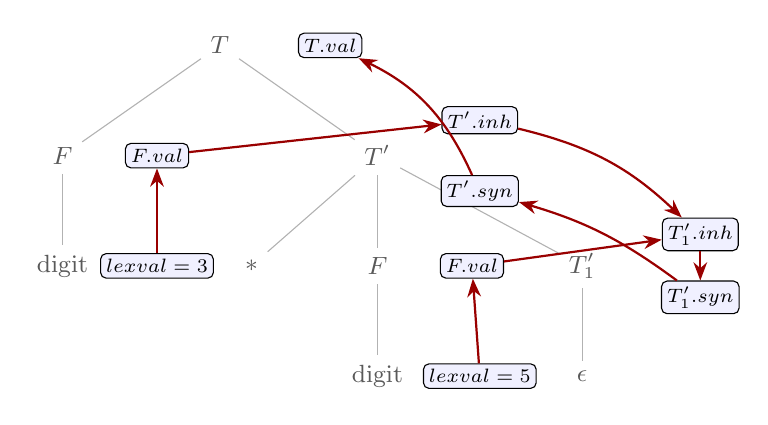
\begin{tikzpicture}[>=Stealth,font=\small,
 tn/.style={font=\small,gray!70!black},
 att/.style={draw,rounded corners=2pt,fill=blue!6,inner sep=2pt,font=\scriptsize},
 te/.style={gray!60,thin}]
% parse tree skeleton
\node[tn] (T) at (3,4.4) {$T$};
\node[tn] (F1) at (1,3.0) {$F$};
\node[tn] (T1) at (5,3.0) {$T'$};
\node[tn] (d1) at (1,1.6) {digit};
\node[tn] (st) at (3.4,1.6) {$*$};
\node[tn] (F2) at (5,1.6) {$F$};
\node[tn] (T2) at (7.6,1.6) {$T_1'$};
\node[tn] (d2) at (5,0.2) {digit};
\node[tn] (ep) at (7.6,0.2) {$\epsilon$};
\foreach \a/\b in {T/F1,T/T1,F1/d1,T1/st,T1/F2,T1/T2,F2/d2,T2/ep} \draw[te] (\a) -- (\b);
% attribute instances
\node[att] (Tval) at (4.4,4.4) {$T.val$};
\node[att] (F1val) at (2.2,3.0) {$F.val$};
\node[att] (d1lex) at (2.2,1.6) {$lexval=3$};
\node[att] (T1inh) at (6.3,3.45) {$T'.inh$};
\node[att] (T1syn) at (6.3,2.55) {$T'.syn$};
\node[att] (F2val) at (6.2,1.6) {$F.val$};
\node[att] (d2lex) at (6.3,0.2) {$lexval=5$};
\node[att] (T2inh) at (9.1,2.0) {$T_1'.inh$};
\node[att] (T2syn) at (9.1,1.2) {$T_1'.syn$};
\draw[->,thick,red!60!black] (d1lex) -- (F1val);
\draw[->,thick,red!60!black] (F1val) -- (T1inh);
\draw[->,thick,red!60!black] (d2lex) -- (F2val);
\draw[->,thick,red!60!black] (F2val) -- (T2inh);
\draw[->,thick,red!60!black] (T1inh) to[bend left=15] (T2inh);
\draw[->,thick,red!60!black] (T2inh) -- (T2syn);
\draw[->,thick,red!60!black] (T2syn) to[bend right=10] (T1syn);
\draw[->,thick,red!60!black] (T1syn) to[bend right=20] (Tval);
\end{tikzpicture}
\end{document}
